\documentclass[c,11pt,xcolor=dvipsnames, aspectratio=169]{beamer}

%Insert number of slides
\beamertemplatenavigationsymbolsempty
\addtobeamertemplate{navigation symbols}{}{%
    \usebeamerfont{footline}%
    \usebeamercolor[fg]{footline}%
    \hspace{1em}%
    \insertframenumber/\inserttotalframenumber
}

% Redefine itemize
\def\labelitemi{--}


%Define colors useful for presentation
\definecolor{UniBlue}{RGB}{0,102,204}
\definecolor{UniOrange}{RGB}{255,128,0}
\definecolor{mygreen}{RGB}{120,190,33}
\newcommand{\green}[1]{\textcolor{ForestGreen}{#1}}

%\definecolor{color1}{HTML}{B3E2CD}
%\definecolor{color2}{HTML}{FDCDAC}
%\definecolor{color3}{HTML}{CBD5E8}
%\definecolor{color4}{HTML}{F4CAE4}
%\definecolor{color5}{HTML}{E6F5C9}

%\definecolor{color1}{HTML}{66C2A5}
%\definecolor{color2}{HTML}{FC8D62}
%\definecolor{color3}{HTML}{8DA0CB}
%\definecolor{color4}{HTML}{E78AC3}
%\definecolor{color5}{HTML}{A6D854}

\definecolor{color1}{HTML}{1B9E77}
\definecolor{color2}{HTML}{D95F02}
\definecolor{color3}{HTML}{7570B3}
\definecolor{color4}{HTML}{E7298A}
\definecolor{color5}{HTML}{66A61E}


\setbeamercolor{title}{fg=color1}
\setbeamercolor{frametitle}{fg=color1}
\setbeamercolor{structure}{fg=color3}
\setbeamercolor{footline}{fg=black}
\setbeamercolor{caption name}{fg=black}
\setbeamercolor{bibliography item}{fg=black}
\setbeamercolor*{bibliography entry title}{fg=black}
\setbeamercolor*{bibliography entry author}{fg=black}
\setbeamercolor*{bibliography entry location}{fg=black}
\setbeamercolor*{bibliography entry note}{fg=black}


\setbeamertemplate{section in toc}[sections numbered]
\setbeamertemplate{caption}[numbered]
\setbeamertemplate{bibliography item}{\insertbiblabel}

%Additional packages
\usepackage{blkarray}
\usepackage{amsmath}
\usepackage{amsfonts}
\usepackage{amssymb}
\usepackage{algorithm2e}
\usepackage{appendixnumberbeamer}
\usepackage{pgfplots}
\usepgfplotslibrary{groupplots,dateplot}
\usetikzlibrary{patterns,shapes.arrows}
\pgfplotsset{compat=newest}
\usepackage{multimedia}
\usepackage{media9}
\usepackage{pbox}
\usepackage{multirow}
\usepackage[makeroom]{cancel}
\usepackage[export]{adjustbox}
\usepackage{tabularx}
\usepackage{caption}
\usepackage{xcolor}
\usepackage{pgfplotstable,filecontents}
\usepackage{listings}
\usepackage{enumitem}
\usepackage{algorithmic}

\usepackage{tikz}
\usetikzlibrary{shapes.geometric, arrows}

\tikzstyle{process} = [rectangle, rounded corners, minimum width=3cm, minimum height=1cm, text centered, draw=black, fill=color1]
\tikzstyle{arrow} = [thick,->,>=stealth]

%GANTT Stuff
\usepackage{pgfgantt}
\newgantttimeslotformat{stardate}{% \def\decomposestardate##1.##2\relax{%
\def\stardateyear{##1}\def\stardateday{##2}% }% \decomposestardate#1\relax%
\pgfcalendardatetojulian{\stardateyear-01-01}{#2}% \advance#2 by-1\relax%
\advance#2 by\stardateday\relax%
}


\newganttlinktype{rdldr*}{%
  \draw [/pgfgantt/link]
    (\xLeft, \yUpper) --
    (\xLeft + \ganttvalueof{link bulge 1} * \ganttvalueof{x unit},
      \yUpper) --
    ($(\xLeft + \ganttvalueof{link bulge 1} * \ganttvalueof{x unit},
      \yUpper)!%
      \ganttvalueof{link mid}!%
      (\xLeft + \ganttvalueof{link bulge 1} * \ganttvalueof{x unit},
      \yLower)$) --
    ($(\xRight - \ganttvalueof{link bulge 2} * \ganttvalueof{x unit},
      \yUpper)!%
      \ganttvalueof{link mid}!%
      (\xRight - \ganttvalueof{link bulge 2} * \ganttvalueof{x unit},
      \yLower)$) --
    (\xRight - \ganttvalueof{link bulge 2} * \ganttvalueof{x unit},
      \yLower) --
    (\xRight, \yLower);%
}
\ganttset{
  link bulge 1/.link=/pgfgantt/link bulge,
  link bulge 2/.link=/pgfgantt/link bulge}
  
\hyphenation{in-com-press-ible}
\hyphenation{com-press-ible}

\newcommand{\link}[3][blue]{\hyperlink{#2}{\color{#1}{#3}}}%



\newcommand\Dganttbar[4]{%
  \ganttbar{#1}{#3}{#4}\ganttbar[inline,bar label font=\footnotesize]{#2}{#3}{#4}
}
% End of GANTT stuff



%Shading text: useful to highlight information
\usepackage{framed, color}
\definecolor{shadecolor}{RGB}{220,220,220}
\usepackage{makecell}

\usepackage{subcaption}
%Define logos for subojectives
% \newcommand{\logoso1}{\setbeamertemplate{logo}{\includegraphics[width=0.1\textwidth]{images/so1.png}}
\def\mathunderline#1#2{\color{#1}\underline{{\color{black}#2}}\color{black}}


\usepackage{siunitx}

% Add an outline slide at the beginning of each new section
\AtBeginSection[]
{
	{
		\setbeamertemplate{footline}{} %this line removes slides numbers
		\begin{frame}[noframenumbering]
			\frametitle{Outline}
			\tableofcontents[currentsection]
		\end{frame}
	}
}




%-------------------------
% Title page
%-------------------------
% Details for title page
% Commenting the line below will make the title page centered
\setbeamertemplate{title page}[default][left,colsep=-4bp,rounded=true,shadow=\beamer@themerounded@shadow]

\title{\textbf{GIT}}
\subtitle{Let's talk about version control}
\author{Bruno \textit{problembär} Blais}


% Logo of the laboratory and the university
\titlegraphic{
\includegraphics[width=4.2cm]{../../logos/chaos_logo_black_without_bkg.png}\hspace*{6.8cm}~%
   
\includegraphics[width=3cm]{../../logos/Polytechnique_signature-RGB-droite_ENG.png}
}



\begin{document}

% Title slide
{
\setbeamertemplate{footline}{} %this line removes slide number
\begin{frame}[noframenumbering]
  \titlepage
\end{frame}
}

%%Contents slide
\begin{frame}
	\frametitle{\textbf{Outline}}
	\tableofcontents
\end{frame}

%% Other slides
\section{Motivation behind this small training session}

\begin{frame} {This has happened to you}

	\begin{figure}[ht]
		\centering
		
\includegraphics[width=1\textwidth]{images/many_vers.jpg}
	\end{figure}


	\visible<2->
	{
Now imagine you want to rerun the homework code and nothing works...
	}
\end{frame}

\begin{frame} {...}
	\begin{figure}[ht]
		\centering
		\includegraphics[width=0.75\textwidth]{images/ctrl_z.png}
	\end{figure}
\end{frame}


\begin{frame} {This is what version control enables}

	\begin{figure}[ht]
		\centering
		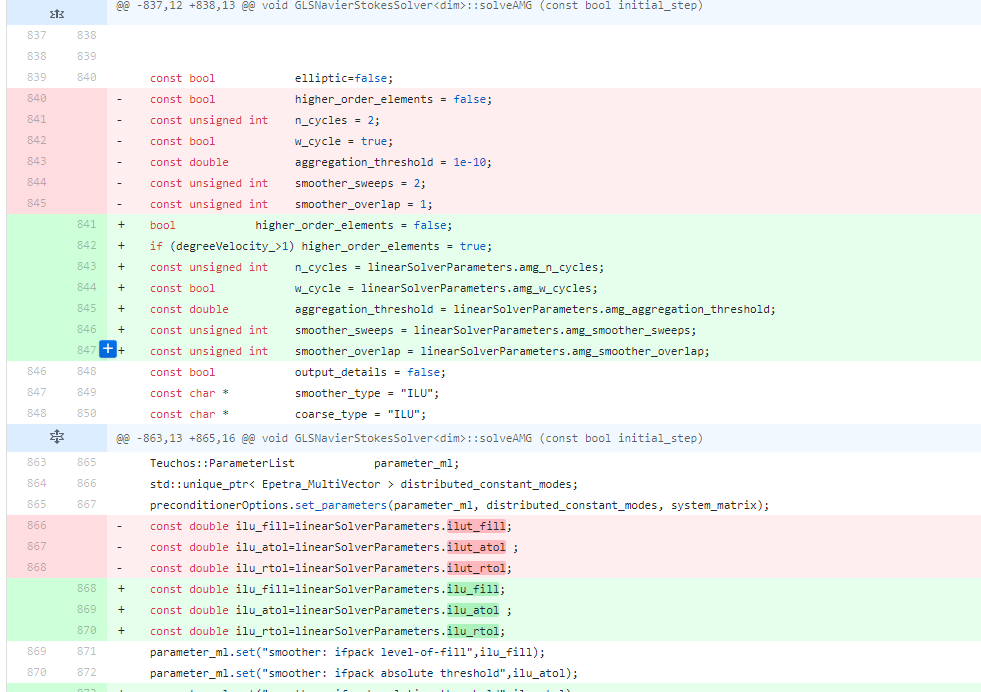
\includegraphics[width=0.65\textwidth]{images/version_control_ex.png}
	\end{figure}


	{
Version control maintains history of the whole project with all changes monitored.
	}
\end{frame}

\begin{frame} {We need to move away from backups...}
\begin{block}{Errors}
Difficult to identify when things worked and when they did not.
\end{block}

\begin{block}{Teamwork}
Incompatible with working as part of a team. 
\end{block}

\begin{block}{Unsustainable}
Incompatible with maintaining / sharing a project in the long term.
\end{block}

\begin{block}{Open-source}
	Incopmatible with the idea of working in open-source.
\end{block}
\end{frame}


\begin{frame} {Version control}
\begin{block}{A mindset}
Version control is not about the tool, it is first about changing your \textbf{mindset}. If you do not change the way you work, this training and the tools are useless.
\end{block}


\visible<2->
{
\begin{block}{Reaping the benefits}
Version control will enable you to structure your mind and forces you to establish steps along your development process.
\end{block}
}
\end{frame}


\begin{frame} {When should I use version control?}

\begin{block}{Good for}
\begin{itemize}
\item software
\item scripts (python, julia, matlab, etc.)
\item articles and slides (if written in \LaTeX)
\item experimental data (if the size is below 1MB)
\end{itemize}
\end{block}
	
\begin{block}{Bad for}
\begin{itemize}
\item images, movies and media
\item binary files (word files, powerpoint, excel, etc.)
\end{itemize}
\end{block}
\end{frame}

\section{Version control and GIT}

\begin{frame}[fragile]{What is a distributed version control system (DVCS)?}

\begin{block}{Version control system}
	\begin{itemize}
	\item Saves all changes to files or file batches
	\item Allows you to go back in time
	\item Merge the work of several people at the desired moment
	\end{itemize}
\end{block}

\begin{block}{Distributed}
	The story is stored on each computer that has a copy of the repository.
\end{block}


\begin{block}{Online}
	\begin{itemize}
		\item Github
		\item Gitlab
		\item Bitbucket
		\end{itemize}
\end{block}

\end{frame}


\begin{frame}[fragile]{What is GIT?}

	\begin{block}{GIT}
 GIT is a DVCS. It is not the only one there is, but it is by far the most popular. It is used to host multiple large project (e.g. the Linux Kernel, etc.)
	\end{block}

	\begin{block}{There are alternative}
		\begin{itemize}
			\item Mercurial (Hg)
			\item Subversion (SVN, this is old)
		\end{itemize}
	\end{block}


	\visible<2->{
		\textbf{In all honesty, GIT is not the easiest DVCS to learn, but since it is by far the most popular, it is better to learn it.}
	}
	
	\end{frame}


\section{Installing GIT and creating a github repository}

\begin{frame}{Installing GIT}

\textbf{Two main ways...}

\begin{block}{Command-line interface}
Generally how most programmers work using GIT. This has a steeper learning curve, but enables you to use all of the features of GIT. On Linux and Mac OS this is generally already installed (or can easily be installed on your machine), on windows it is easier if you use WSL.
\end{block}

\begin{block}{Graphical user interface}
There are many graphite user interface for GIT. Today I will show you mainly \textbf{github desktop}, but many alternative exist.
\end{block}


\end{frame}



\section{Using GIT on a single branch}

\begin{frame}{Creating a remote repositoy}

	Let's create a repository together:
	\begin{itemize}
	\item Create Github account (or login to existing one)
	\item Create an empty repository
	\item Clone repository on your machine
	\end{itemize}
\end{frame}

\begin{frame}[fragile]{Main steps in using GIT}
	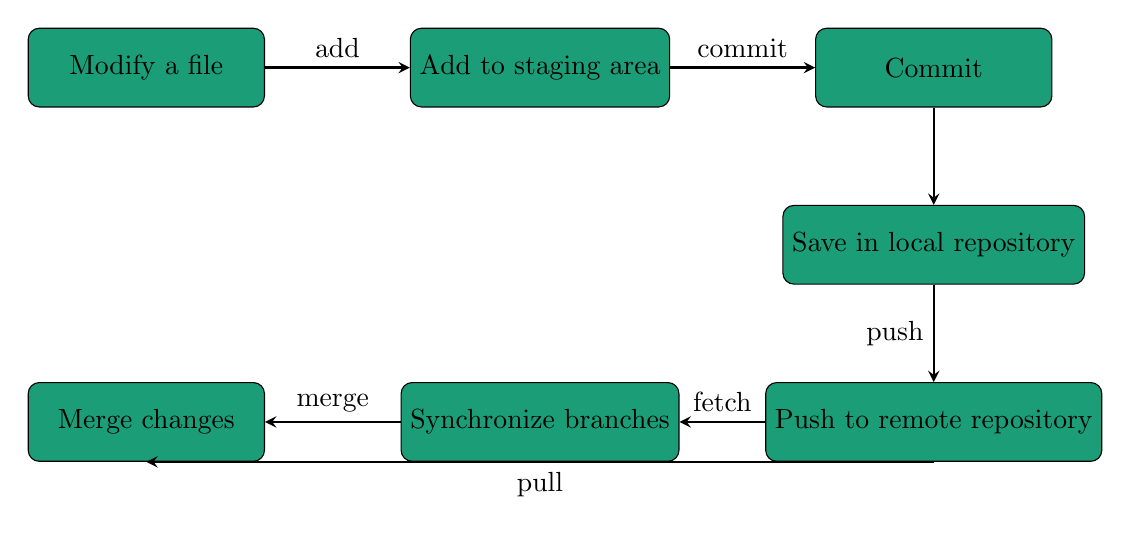
\begin{tikzpicture}[node distance=2cm]

		\node (modify) [process] {Modify a file};
		\node (stage) [process, right of=modify, xshift=3cm] {Add to staging area};
		\node (commit) [process, right of=stage, xshift=3cm] {Commit};
		\node (local) [process, below of=commit, yshift=-0.25cm] {Save in local repository};
		\node (push) [process, below of=local, yshift=-0.25cm] {Push to remote repository};
		\node (sync) [process, left of=push, xshift=-3cm] {Synchronize branches};
		\node (merge) [process, left of=sync, xshift=-3cm] {Merge changes};
		%\node (fetch) [process, right of=sync, xshift=3cm] {Fetch};
		%\node (pull) [process, right of=fetch, xshift=3cm] {Pull};
		
		\draw [arrow] (modify) -- node[anchor=south] {add} (stage);
		\draw [arrow] (stage) -- node[anchor=south] {commit} (commit);
		\draw [arrow] (commit) -- node[anchor=east] {} (local);
		\draw [arrow] (local) -- node[anchor=east] {push} (push);
		\draw [arrow] (push) -- node[anchor=south] {fetch} (sync);
		\draw [arrow] (sync) -- node[anchor=south] {merge} (merge);
		\draw [arrow] (push.south) --   node[anchor=north] {pull} (merge.south);
		
		\end{tikzpicture}
\end{frame}


\section{Using GIT with multiple branches}

\begin{frame}[fragile]{Branches: working as a team}
	\begin{figure}[ht]
		\centering
		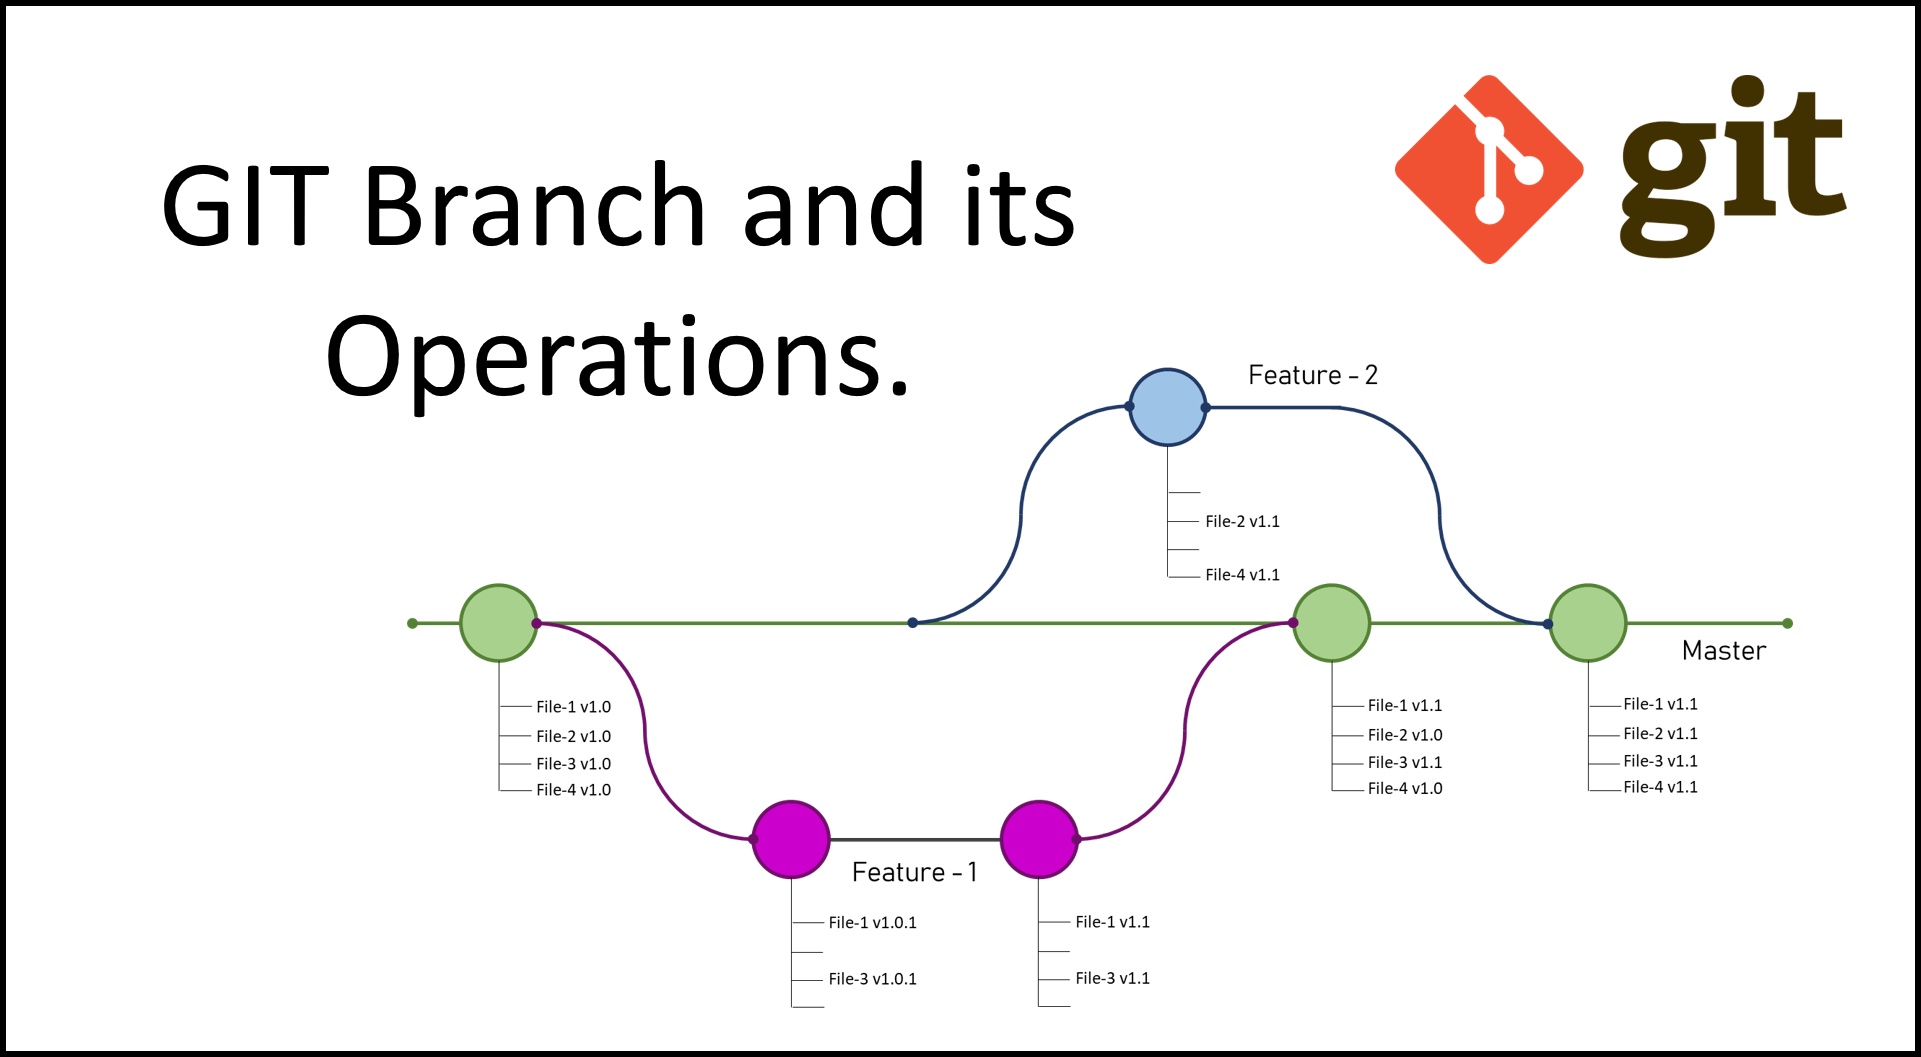
\includegraphics[width=1\textwidth]{images/branches.png}
	\end{figure}
\end{frame}


\begin{frame}[fragile]{Let's use branches together}
	Let's do the following:
	\begin{itemize}
	\item Create a branch
	\item Modify a file
	\item Commit the changes
	\item Do another change and commit
	\item Merge branch on main
	\end{itemize}
\end{frame}


\begin{frame}[fragile]{Pull requests: how it works in practice!}
In real life, you will not be alone working on your code. It is best practice to not merge to \textbf{main} your changes directly, but instead, go through a review process. 

\visible<2->
{
	\begin{block}{Pull request!}

		Pull request enable you clearly state the changes you wish to make to the main version of the code.
		\begin{itemize}
		\item Allows others to review it 
		\item Allows for easy continuous integration
		\end{itemize}

	\end{block}
}

\end{frame}

\section{Conclusion: the end}

\begin{frame}{Conclusions}
\begin{block}{GIT and version control}
	\begin{itemize}
	\item Essential if you want to work as part of a team
	\item Allows you to track every change and go back in time (e.g. git bissect)
	\item Allows you to share your code with who you want in a safe and controllable way.
	\end{itemize}
\end{block}

\begin{block}{You need to change the way you work}
	\begin{itemize}
	\item When you start a new feature, create a branch and work on it.
	\item Aim for small features, once they are complete, merge them.
	\item Don't be afraid of criticism, getting comments is a good way to get better.
	\end{itemize}
\end{block}
\end{frame}


\begin{frame}{Advices for the future}

	\begin{block}{Above all things, using git requires discipline}
		\begin{itemize}
		\item If you can name an idea or a change, it should be a branch and a pull request.
		\item Ensure you have ways to test your changes. Automating these tests is easier than you think (e.g. use continuous integration)
		\item Write clear commit messages and pull request messages. It is a small time investment that can save you a lot of time and it structures your ideas.
		\item Do not be afraid of failing or making mistake, git enables you to go back in time, so you CAN do large-scale refactoring.
		\end{itemize}
	\end{block}

	\begin{block}{There is more to git...}
		\begin{itemize}
		\item Rebase
		\item Cherry-picking
		\item Squashing
		\item ... (many other things I do not know)
		\end{itemize}
	\end{block}

\end{frame}

\end{document}